\documentclass[11pt]{article}
\usepackage{deauthor,times,graphicx}

\usepackage{amsmath,amssymb,amsfonts}
\usepackage{newtxtext,newtxmath}
\usepackage{url}
\usepackage{xspace}

\usepackage{graphicx}
\usepackage{textcomp}
\usepackage{xcolor}

\newcommand{\affone}{\textsc{AffC}\xspace}
\newcommand{\affall}{\textsc{AffD}\xspace}
\newcommand{\lpone}{\textsc{LpD}\xspace}
\newcommand{\lpall}{\textsc{LpA}\xspace}
\newcommand{\affs}{\textsc{Aff-*}\xspace}
\newcommand{\lps}{\textsc{Lp-*}\xspace}
\newcommand{\gafonelpone}{\textsc{GrAffC-LpD}\xspace}
\newcommand{\gafonelpl}{\textsc{GrAffC-LpA}\xspace}
\newcommand{\gafllpone}{\textsc{GrAffD-LpD}\xspace}
\newcommand{\gafllpl}{\textsc{GrAffD-LpA}\xspace}
\newcommand{\nord}{\mbox{\sc{NoOrder}}\xspace}
\newcommand{\total}{\mbox{\sc{TotalOrder}}\xspace}
\newcommand{\pord}{\mbox{\sc{PartialOrder}}\xspace}
\newcommand{\alter}{\mbox{\sc{Alternate}}\xspace}
\newcommand{\eat}[1]{}

\begin{document}
\title{An ML-Powered Human Behavior Management System}
\author{Sihem Amer-Yahia$^*$, Reynold Cheng$^+$, Mohamed Bouadi$^*$,
Abdelouahab Chibah$^*$,\\ Mohammadreza Esfandiari$^*$, 
Jiangping Zhou$^+$, Nan Zhang$^+$, Eric Lau$^+$, Yuguo Li$^+$,\\
Xiaolin Han$^+$, Shivansh Mittal$^+$\\
$^*$Univ. Grenoble Alpes, CNRS, France,\\ \{firstname.lastname\}@univ-grenoble-alpes.fr\\ $^+$University of Hong Kong, ckcheng@cs.hku.hk,\\
\{zhoujp, liyg, zhangnan,
ehylau, xiaolinh, shivansh\}@hku.hk
}
\maketitle

\date{}


\begin{abstract}
Our work aims to develop novel technologies for building an efficient data infrastructure as a backbone for a human behavior management system. Our infrastructure aims at facilitating behavior modeling, discovery, and exploitation, leading to two major outcomes: a behavior data management back-end and a high-level behavior specification API that supports mining, indexing and search, and AI-powered algorithms that provide the ability to extract insights on human behavior and to leverage data to advance human capital. We discuss the role of ML in populating and maintaining the back-end, and in exploiting it for human interest. 
\end{abstract}

\section{Introduction}
We make a case for building a human behavior management system, where human behavior is a first class citizen and is mined, queried and managed over time. While several efforts have focused on studying human behavior in large scale population studies, in mining customer purchase patterns, or on the social Web, there is no single architecture that provides the ability to mine, query and manage behavior. Such a system would encourage reproducibility and enable several applications that benefit humans. In particular, the ability to model individual and collective behavior enables to offer new functionalities that let everyone can share and discover all kinds of assets, and combine assets to advance  human capital. Assets can be composed into learning strategies that everyone can use to propose their skills, acquire new skills, or enhance existing ones.  The proposed research will contribute to designing and developing approaches that leverage ML for building an effective and efficient human behavior management back-end that represents the variety of behaviors and caters to human needs. To enable this work, two novel and challenging research axes need to be developed in parallel: a database system to manage human behavior and a set of ML-powered algorithms that populate and maintain that database, as well as approaches to search and leverage behavior and assets with the goal of studying human behavior and advancing their capital.

To design a human behavior database, we need to capture human factors and populate the database by mining behavioral patterns over time. We propose to leverage approaches that estimate human factors~\cite{RTR+15} and mine behaviors at the individual and collective levels~\cite{DBLP:conf/vldb/KiferBG04, ijcai2017-336, miglausch2000thoughts}. The highly dynamic nature of human factors and behavior renders the maintenance of such a database quite challenging. We propose to leverage ML approaches to (i) learn behavior change rates, (ii) develop adaptive approaches to cater to humans, and (iii) choose back-end maintenance strategies accordingly.
Existing work that leverages ML for data management~\cite{DBLP:conf/sigmod/Stoica20} is nascent and covers the use of ML for query optimization~\cite{DBLP:conf/sigmod/KristoVCMK20} or for database indexing~\cite{DBLP:conf/sigmod/KraskaBCDP18}. Additionally, the ability to search and leverage behavior and assets with the goal of studying human behavior and advancing their capital requires the development of novel ML-powered algorithms. 

To study human behavior, we plan to develop a flexible tool for the on-demand discovery of behavioral patterns and their exploration over time. Such functionality benefits a variety of stakeholders. It would enable the design of robust population studies, marketing strategies, and promotional campaigns. Data scientists, social scientists, Web application designers, marketers, and other domain experts, need a single destination to explore behavioral changes.
To query human behavior, we will leverage work on querying time series. Systems like Qetch~\cite{DBLP:conf/sigmod/ManninoA18} and ShapeSearch~\cite{DBLP:conf/sigmod/SiddiquiLWKP20} provide the ability to express powerful shape queries through sketches, natural language, and regular expressions with flexible time span and amplitude. However, those queries are solely shape-based and cannot be used to search for change induced by humans of interest. We will hence develop approaches to combine shape queries with querying humans and change intensity.

For leveraging assets to advance human capital, we will make use of recent work on virtual marketplaces~\cite{DBLP:conf/kdd/EsfandiariWAR19}. In physical workplaces, learning strategies include scaffolding where assets are combined in alternating difficulty levels, and collaboration where humans learn from their interactions with higher-skilled peers~\cite{DLL+17,KH13,LL89}. In virtual marketplaces, a few studies focused on humans' ability to improve their skills by completing tasks~\cite{GD17}, and how affinity between humans can be used to form teams that collaborate to produce high quality contributions while also improving skills~\cite{DBLP:conf/kdd/EsfandiariWAR19}. Our observation is that optimizing for human capital should be seen as a multi-objective problem that accounts for several goals and quality control, cost reduction, and human effort. We will develop a framework to observe humans and leverage ML techniques to learn their abilities and adaptively suggest appropriate assets to them for advancing their capital while accounting for other goals.

\section{Motivating examples}

\begin{example}[Mining and querying behavior.]\label{ex1}
Our first example motivates the need for sophisticated mining approaches to discover and model evolving human behavior. We consider two typical examples: mining customer behavior in retail and mining the behavior of citizens riding public transportation. Mining behavior can help identify purchase patterns in the first case, and specific rider groups in the second, e.g., familiar stranger groups who use public transportation during the same period. In both examples, evolving behavior captures changing habits such as customers reacting to promotional offers, or riders changing groups when in transit. The ability to query behavior changes is useful for people in charge to analyze usage trends. In the riders case, this would help them identify trends of daily travel populations over time and see their behaviors change when special events occur (e.g., during the COVID-19 crisis). Extracted insights must be made available through a powerful querying interface to instruct public policies (e.g., new COVID-19 measures). Additionally, they can be used to train behavior change models that will instruct data maintenance. By learning different change models, we will enable ML-powered back-end updates.
\end{example}

\begin{example}[Assets for advancing capital.]\label{ex2}
Assets such as online courses or facts to be verified, can be used for advancing human capital and the system must help humans improve their skill and knowledge either individually or collaboratively (a.k.a. peer learning).
Assume we have 3 humans: Mary, John and Sarah. Mining their behavior in an online course system would help determine their skill level (1 for Mary who is a novice, 3 for John who has an intermediate level, and 5 for Sarah who is an expert). Given the courses they consumed so far, our goal is to assign to Mary a batch of $k=5$ assets that maximize her learning. Mary needs the support of John or Sarah to consume intermediate level assets. She cannot consume hard assets even with help. By exposing Mary to her peers' contributions, her learning potential is likely to increase~\cite{DKK+12}. Assigning over-challenging assets to her may result in frustration, and assigning under-challenging assets may lead to boredom.

In another example, we have a set of fact-checking tasks. Each task constitutes a collaborative asset, to be consumed by $12$ individuals with varying skills.  Each pair of individuals has an affinity that reflects how effectively they can collaborate based on their socio-demographics. Therefore, there are $12 \choose 2$ pairs of affinities forming a graph. One goal here is to divide the humans into $3$ equi-sized groups of $4$ members each so that peer learning is maximized.
\end{example}

\section{Our system}

\subsection{Building a human behavior management database} 
The goal of this axis is to develop an
integrated data model to represent human behavior, encompassing  human factors and asset dimensions, and to leverage ML in maintaining the database. To make behavior and assets usable, we need to develop an API for populating, maintaining and accessing 
behavior and assets, including a declarative query language for expressing
complex conditions on human factors and behavior and assets. Through these objectives it will
be possible to offer querying human behavior and assets as a simple service promoting their 
reusability. Additionally, we will
investigate performance aspects of this language and propose
mechanisms for its efficient evaluation. The database needs to store raw human/asset data but also the results of extracting insights such as mining behavioral change of user groups. The evolving nature of human
factors makes this particularly challenging. It is therefore necessary to apply ML approaches to learn behavioral change models and leverage them at maintenance time, when new raw data and new insights need to be stored in the back-end. This ML-powered approach will be compared against traditional batch and incremental maintenance approaches.  

{\bf Objectives:}
\begin{enumerate}
\item Design a model to capture, represent and manage human factors, human behavior and assets. Two kinds of factors must
be considered: people-specific ones such as socio-demographic attributes, skill,
reputation/trust, and motivation;
and collaborative factors such as affinity and interaction
models. 
\item Design a model to capture and store extracted insights on individual and group behavior.
\item Investigate indexing mechanisms to retrieve and query  
behavioral change and assets efficiently.
\item Develop ML-powered algorithms for updating and
managing evolving human behavior at individual and group levels.
\end{enumerate}

\subsection{Leveraging assets} 
This axis explores the study and querying of human behavior over time and the development of approaches for leveraging assets in different applications. In particular, we will focus on leveraging assets for advancing human capital. In our first endeavor, we will design queries that express behavior-aware change primitives. Our queries will be sent to the backend and need to be expressive enough to query behavior shapes and changes. This would require defining new scoring semantics that combine shape matching and intensity of change. Existing algorithms to match shape queries operate in time series and rely on splitting time using a fixed-size window and matching the query to each region in the window. We will leverage drift detection approaches on data streams~\cite{DBLP:conf/vldb/KiferBG04} to handle time in a dynamic fashion. 

In our second endeavor, we will study asset assignment, expecting that appropriate assignments will have a positive impact on the inherent learning capability of humans and on their overall performance.
We focus on a common class of assets, ``Knowledge assets'' in Bloom's taxonomy of educational objectives~\cite{Bloom56,KA09} such as image classification, text editing, labeling, fact checking, and speech transcription asset. A common problem we will tackle is: 
given a human $h$ and a set of unconsumed assets, which sequence of $k$ assets will maximize $h$'s learning potential? Here, learning potential is the maximum possible improvement in $h$'s skill.

We adopt a model where contributions from other humans are made visible to the current human. Several studies showed that humans learn better when contributions from higher-skilled humans are shown to them~\cite{DMB+14,DKB19,KIM15,KMM+18}. Our challenges are:
(1) how to choose an appropriate batch of $k$ assets where a human can see others' contributions, (2) how to order the chosen $k$ assets appropriately so that the human's skill improvement is maximized. Our approach must enabke both individual and peer learning. We will leverage work in online critiquing
communities,\footnote{\url{https://movielens.org/}} social Q\&A
sites,\footnote{\url{http://quora.com/}} and crowdsourcing
platforms\footnote{\url{https://www.figure-eight.com/}} that investigate how collaboration can promote knowledge and skill improvement of individuals. In particular, we propose
to explore how affinity between group members improves peer
learning and address modeling, theoretical, and algorithmic challenges. We will build on our recent work for algorithmic group formation with
affinities for peer learning~\cite{DBLP:conf/kdd/EsfandiariWAR19}.

%\begin{figure}[htpb]
%    \centering
%    \begin{minipage}{.5\textwidth}
 %       \centering
  %      \includegraphics[width=0.4\columnwidth]{figs/zpf.png}
   % \caption{Zone of Proximal Flow~\cite{BRK+13}, which combines the results of ZPD and Flow Theory.}
    %\label{fig:zpf}
    %\end{minipage}%
    %\begin{minipage}{0.5\textwidth}
     %   \centering
      %   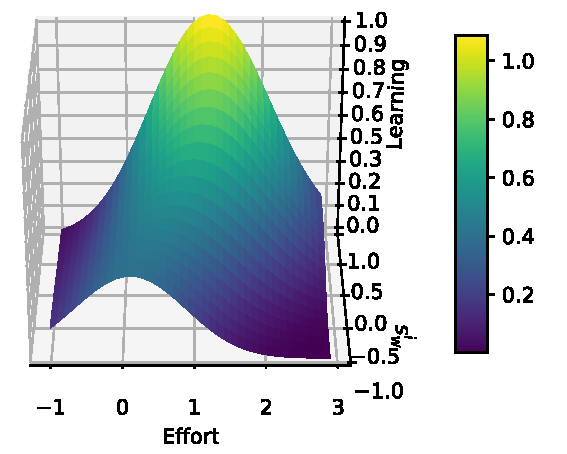
\includegraphics[width=0.6\columnwidth]{figs/Learning3d.pdf}
    %\caption{Learning potential distribution}
    %\label{fig:learning}
    %\end{minipage}
%\end{figure}

{\bf Objectives for querying behavior:}
\begin{enumerate}
  \item Formalize an algebra that captures behavior evolution over time.
  \item Develop a framework that given raw human/asset data, extracts groups and their behavior, stores them as insights in the database and represents change using our algebra.
  \item Build a visual interface to query behavior with powerful conditions on behavior shape and change intensity.
\end{enumerate}

{\bf Objectives for learning:}
\begin{enumerate}
  \item Formalize the {\it learning potential} of a human for an asset and choose $k$ assets that maximize the total learning potential. This formalization should capture individual learning and peer learning.
There are two theories underlying our framework.
First, Zone of Proximal Development (ZPD)~\cite{VYG87} is a well-known theory that defines three zones of assets with different skill improvements; (1) A learnable zone that contains assets a person can learn how to consume when assisted by a teacher or peer with a higher skillset, (2) a flow/comfort zone of assets that are easy and can be consumed with no help, and (3) a frustration zone of assets that a learner cannot consume even with help.
Second, the Flow theory~\cite{CSI75} states that people are able to immerse themselves in doing things whose challenge matches their skills. %Figure~\ref{fig:zpf} integrates the two theories and illustrates their relationship with respect to the asset challenge, the user skill, and the affect state~\cite{BRK+13,MAT17}.
In~\cite{BRK+13}, the authors claim that to improve skills, the assets should be either in the flow/comfort zone, or in the learnable zone on the condition that there is some ``scaffolding'' to help humans consume assets that are a bit more challenging for them. This results in skill improvement (the dotted line).
Our formalization builds on that and defines the learning potential for both individual assets (mainly in the flow/comfort zone) and collaborative assets (mainly in the learnable zone).

\item Devise learning strategies which interleave individual assets and collaborative assets. We will study their impact on humans' performance and skills. Previous work found that the order of assets impacts quality and completion time~\cite{DRP+15,CIT16}. For instance, assets could be provided in no particular order, or grouped and presented in alternating difficulty levels. 

\item Propose adaptive and iterative asset search methods that take a human $h$, and assigns to $h$, at each iteration, a batch of $k$ assets according to a learning objective. This approach may give rise to multi-objective problems.
\end{enumerate}

\section{Modeling human behavior}
Our model must capture humans, assets, and human behavior and its evolution over time. 
Figure~\ref{fig:ER} shows a two-level E/R diagram that represents human and asset data and extracted insights. It will serve as a basis for the design of our backend.

\begin{figure}[htpb]
    \centering
        \includegraphics[width=0.8\columnwidth]{submissions/reynold/figs/ER.jpg}
    \caption{E/R diagram representing raw human/asset data and extracted insights.}
    \label{fig:ER}
\end{figure}

The above framework could be used to discover and model evolving human behavior of citizens riding public transportation, and see how their behaviors change when special events occur. Here, we aim to study passenger behaviors during the COVID-19 crisis. COVID-19 is characterized by a broad spectrum of disease presentation, from asymptomatic or subclinical infections to severe diseases and deaths. A person infected with SARS-CoV-2 virus who has not yet developed symptoms or confirmed by laboratory testing would likely maintain normal social activities. Recent studies show that infected cases are contagious for asymptomatic and pre-symptomatic cases, and continuous to be contagious for at least a week~\cite{lau20, emery20}, providing ample opportunity for transmitting SARS-CoV-2 through public transportation. Recently, we have performed a study in Hong Kong with the Mass Transit Railway (MTR) Corporation, which is the only railway and subway service provider in Hong Kong.  The MTR railway network covers areas inhabited by more than 70\% of the local population~\cite{housing14}.  About 50\% of total number of rider trips in Hong Kong (or 4.5 million riders) are made through MTR~\cite{transport17}.  Thus, the local population mobility in Hong Kong is well represented by the MTR traveling population. Courtesy of MTR, we have obtained {\it all} the entry and exit data of of anonymous riders (e.g., time and station of entry, ticket type (kid/adult/elder)) in the first four months (i.e., 1 January to 30 April) of 2020, which is also a coronavirus outbreak period in Hong Kong. 

We have performed some initial analysis of the MTR data. Figure~\ref{fig:MTR-trend} shows the change of daily population in the first three months of 2020 (here, {\it octopus} refers to the most popular smart card in Hong Kong; {\it ticket} means the single entry ticket). We can see that the daily MTR traveling population is reduced by more than 40\% after the end of Chinese New Year holiday on Jan 28, which can be related to the lockdown of Hubei, China on Jan 23, just before the holiday. Also, the MTR traveling population in weekends is more than 10\% less than that in workdays. Another observation is that while the number of MTR passengers is generally decreasing, the number of new confirmed cases increases significantly.


\begin{figure}[!hbt]
\centering
\includegraphics[width=0.6\columnwidth,page=1]{submissions/reynold/figs/MTR-trend.pdf}
\caption{MTR daily population and number of infected cases in Jan-Mar 2020.}
\label{fig:MTR-trend}
\end{figure}

%Mining behavior can help identify specific rider groups in the second, e.g., familiar stranger groups who use public transportation during the same period. Evolving behavior captures riders changing groups when in transit. The ability to query behavior changes is useful for people in charge to analyze usage trends. In the riders case, this would help them identify trends of daily travel populations over time and see their behaviors change when special events occur (e.g., during the COVID-19 crisis). Extracted insights must be made available through a powerful querying interface to instruct public policies (e.g., new COVID-19 measures). 

{\bf Rider type discovery.} The MTR riders could physically encounter one another, and temporally share different facilities or spaces such as stations, platforms, elevators, and carriages. They can concurrently share a crowded and small carriage for an extensive amount of time. We would also like to study different group behaviors of MTR riders in the period of January to March 2020, during which the outbreak of coronavirus occurs. As discussed in \cite{zhou2020familiar}, these riders include:

\begin{itemize}
	\item ``Someone-like-you'': they are groups of riders who share the same trip and stay close to each other, and simultaneously share trajectories for at least one trip. 
	
	\item Sensor riders, who have the most physical contacts with other riders at stations and carriages. If they are ``super spreaders'', they can infect many people. 

	\item Extreme riders, who have to endure the longest journeys or who have to ride the MTR train most frequently. They can have a high risk of contracting coronavirus or respiratory diseases.

	\item Choice riders, who quickly change their travel patterns given the COVID-19 situation, for example, due to outbreak in certain districts, or new government policies for work and classes. 

\end{itemize}

We aim to discover the above riders through mining the MTR data. The riders found can be useful to understand whether they have a high risk of spreading or contracting coronavirus.  They can be useful for simulating scenarios and testing rider control and intervention policy. Moreover, they can be used for issuing warning or further actions. For example, in a ``someone-like-you'' group, if any member of this group contracts contagious viruses, other members who are close contacts of the patient should be notified and monitored as soon as possible.  We will develop data mining solutions to identify rider types from the MTR data. For example, to obtain ``someone-like-you'' riders, one way is to group the rider information according to the stations and the times they entered and exited. Each group consists of riders who are estimated to take the same train.  
%To illustrate, Figure~\ref{fig:network_map} shows part of the MTR network. Suppose that two persons, $A$ and $B$, checked in at the ticket gate in the HKU station at 9:28am and 9:30am, then left the Chai Wan station at 10:00am and 10:03am respectively. Then, it is likely that $A$ and $B$ take the same train, belonging to a ``someone-like-you'' group.  
We will study methods for finding all these groups, and perform extensive analysis, including the estimation of average group size over weekdays and weekends, and examining the station-pairs that exhibits large group sizes.  Figure~\ref{fig:HK-familiar} shows the  spatial-temporal patterns of the average ``someone-like-you'' group sizes along different MTR trips during workdays in Hong Kong before Jan 24 and after Jan 28 in 2020. The thickness of the line indicates the size of the rider group. We can see that that the trips with the largest ``someone-like-you'' groups in the two time periods are not the same. We will compare the rider types across the first four months of 2019 and 2020. 

\begin{figure}[!hbt]
	\centering
	\includegraphics[width=\columnwidth]{submissions/reynold/figs/HK-familiar.pdf}
	\caption{Spatio-temporal patterns of ``someone-like-you'' riders in MTR. }
	\label{fig:HK-familiar}
\end{figure}


Due to the gigantic number of riders, the discovery of rider types can be time-consuming. We will develop fast database algorithms and indexes to discover riders efficiently. We will  extend the TopPI algorithm~\cite{DBLP:journals/is/LeroyKTA17}, developed by co-I Amer-Yahia, in order to mine rider groups from millions of records in sub-seconds. We will also extend the work on exploring datasets with rating maps to enable group comparison~\cite{DBLP:conf/www/Amer-YahiaKKLZ17}.

Our initial studies show that the data in hand is very promising (e.g., find out the risks of contracting coronavirus for different groups of passengers, and riders' travel behavior arising from the anxiety of being infected in public transport). However, without a scalable platform for human behavior analysis, it is difficult to perform advanced analysis and simulation. In particular, the MTR data, more than 60GB, contains more than 1 billion entry/exit transactions of 8 million riders. We would like to perform ``microscopic'' analysis (e.g., do riders have a close contact?), and also see how the disease is spread in a crowded train with insufficient ventilation. As the MTR data spans 4  months, it is also interesting to examine how the behaviors of passengers change with time. Existing practices and solutions in the public health and transportation fields are not scalable to handle such a large amount of data (e.g., it takes more than 5 hours to perform a task to analyze rider behavior for a single day's data).  This is simply too slow in face of the crisis that we are facing. The proposed system would be able to support analysis on the group behavior of citizens taking public transportation. Our results would help to monitor population transmission potential, and guide the appropriate level of social distancing measures~\cite{buckee20}.

\section{Leveraging assets for learning}
We consider a set of humans $\mathcal{H}$ and a set of assets $\mathcal{A}$. Humans in $\mathcal{H}$ consume assets in $\mathcal{A}$ at different times, either together or separately. The term asset is general enough to represent recommendations on the social web, courses in an online teaching system, tasks in crowdsourcing, etc. We denote $\mathbf{A}_h^t$ a batch of (possibly ordered) assets consumed by a human $h$ at time $t$. The learning potential of a human $h$ who consumes a batch of assets {\bf A} at time $t+1$ depends on several factors: 1) the effort of $h$ to consume assets in {\bf A}, 2) $h$'s performance factor, 3) other humans' performance when learning collaboratively, and 4) the affinity between $h$ and other humans. This gives rise to two problems: individual learning and collaborative learning.
 
We can define learning as the problem of individual asset assignment as follows:
Given a human $h$ and the batches of assets consumed by $h$ up to iteration $i$: $\mathbf{A}_h^1 \ \ldots \ \mathbf{A}_h^t$, find a batch $\mathbf{A}$ of at most $k$ assets to assign to human $h$ at time $t+1$ such that:

\[ \operatorname*{argmax}_{\mathbf{A}} \mathit{learning}(h,\mathbf{A}) \]

$\mathit{learning}(h,\mathbf{A})$ is a function that captures the learning potential of $h$ who consumes the set of assets $\mathbf{A}$. Our problem is to determine the right batch of assets to provide to a human at time $t$. 
Our problem can be seen as a variant of the Knapsack Problem~\cite{Chekuri06apolynomial}. Our items are assets and each asset has a value (in our case $v$ is $\mathit{learning(w,t)}$) and a weight, we want to find $k$ assets that maximize the sum of values $\sum v_i$ under a capacity constraint $k$. What makes our problem simple is that the weight is equal to 1 which yields a top-$k$ solution. Additionally, as the value of assigning an asset to a human depends on the human and evolves over time as other humans consume assets, we need to account for that dynamicity in the asset assignment process. 

We can also define a variant of our problem where assets are consumed collaboratively:
%We can now define our group formation problem.\\
%\textbf{Problem.}
Given a set $H=\{h_1,...,h_n\}$ of humans with their corresponding skill values $h_t^s$, our goal is to form a grouping $\mathcal{G}$ that contains $k$ equi-sized groups $g_1,g_2,...,g_k$ and that maximizes two objective functions, aggregated learning potential ({\em LP}) and aggregated affinity ({\em Aff}) between humans in the same group. More formally:

\begin{equation}
\begin{aligned}
& \underset{\mathcal{G}}{\text{maximize}}
& & \sum_{i=1}^{k}\mathit{LP}(g_i), \sum_{i=1}^{k}\mathit{Aff}(g_i)
\ \ \text{s.t.} \ \ |\mathcal{G}| = k, \ |g_i| = \frac{n}{k}
%& & &   \\
\end{aligned}
\label{multiobjective-proA}
\end{equation}

where $\mathit{LP}(g_i)$ (resp. $\mathit{Aff}(g_i)$) refers to any of the learning potential (resp. affinity). \\

Since the two objectives are incompatible with one another, our problem qualifies as {\em multi-objective}. 
In~\cite{DBLP:conf/kdd/EsfandiariWAR19}, we present approximation algorithms that find a feasible grouping (that maximizes learning potential) and offer provable constant approximation for affinities. We plan to build on that work.


%\textbf{Skill.} Each human has an approximated skill reflecting an ability to consume an asset. For instance, in crowdsourcing, skills could be inferred from previously completed tasks~\cite{DBLP:journals/pvldb/RahmanTRAD15}. The skill of a human $h$ at time $t$ is denoted $\theta_h^t$. 

%\textbf{Individual learning potential.}
 
 Whenever a human consumes a collaborative asset, the asset's metadata is updated. Additionally, assets are grouped by difficulty level and by the number of remaining humans. 
A human's performance factor and skill also need to be updated as humans consume assets. We assume that a human's skill improves monotonically: the skill level remains the same or increases as time passes~\cite{ML13,UMK20} and is updated as they consume more assets. An ML approach that observes humans and revisits their attributes is warranted. 


%\textbf{Effort.}
%Let $\mathit{effort}(h,a)$ be the function that evaluates the gap between the human skill and the asset difficulty level to reflect the effort $h$ needs to deploy to consume $a$.
%For an asset $a$, 
%$\mathit{effort}(h,a)$ is a function of contributions of other humans $v$ who consumed $a$ so far:

%\[
%\mathit{effort}(h,a) = \theta_a-\frac{\mathrm{min}(\theta_v, \theta_a)+\theta_h}{2}
%\]

%In Example~\ref{ex2}, $\mathit{effort}(\mathrm{Mary},a_6) = 1-1 =0$, %$\mathit{effort}(\mathrm{Mary},a_5) = 3-(3+1)/2 =1$.
%In practice, $\mathit{effort}(h,a)$ is time-dependent and only those humans $v$ who consumed $ct$ will contribute to improving the skill of $h$. 
%We will consider this when we formalize our problem.

%\textbf{Performance.} Let $p_h^t$ be the performance of human $h$ at time $t$. This captures the difference between the {\em expected} performance and the {\em observed} performance of $h$ for a batch of assets {\bf A} at time $t$. 

%$p_h^t \in$ [-1,1] reflects whether the observed performance is better than the expected ($s_h^t$ is close to 1), same ($s_h^t = 0$), or worse ($s_h^t$ is close to -1). $\mathit{observed}(h,\mathbf{A}_h^t)$ is computed as the average performance for assets in $\mathbf{A}_h^t$. We measure performance as a tuple of quality and completion time. These notions can be easily understood in the case where assets are courses or tasks. In other domains, they need to be revisited. 
%\[
%\mathit{observed}(h,\mathbf{A}_h^t)= \langle avg_{a\in\mathbf{A}_h^t}\mathit{quality}(h,a),avg_{a\in\mathbf{A}_h^t}\mathit{time}(h,a) \rangle
%\]

%$\mathit{expected}(h,\mathbf{A}_h^t)$ is computed as the average performance for past assets whose effort level is the same as assets in {\bf A} at time $t$;
%\[
%\mathit{expected}(h,\mathbf{A}_h^t)= \langle avg_{\hat{a}\in\mathbf{\hat{A}}}\mathit{quality}(h,\hat{a}),avg_{\hat{a}\in\mathbf{\hat{A}}}\mathit{time}(h,\hat{a}) \rangle,
%\]

%where $\mathbf{\hat{A}} = \{\hat{a} \ | \ \hat{a} \in \{\mathbf{A}_h^1 \ldots \mathbf{A}_h^{t-1}\}, \theta_{\hat{a}} \simeq \theta_{a\in\mathbf{A}_h^t}\}$.\\

%A human's performance is therefore measured as follows:

%\[
%p_h^t = {\rm erf}({\rm d}(\mathit{observed}(h,\mathbf{A}_h^t),\mathit{expected}(h,\mathbf{A}_h^t))),
%\]

%where erf($x$) is an error function: $${\rm erf}(x) = \frac{2}{\sqrt{\pi}}\int_0^x e^{-t^2}\,\mathrm dt$$
%${\rm d}(\mathbf{p},\mathbf{q})$ is a Euclidean distance
%$${\rm d}(\mathbf{p},\mathbf{q})=\sqrt{(q_1-p_1)^2 + (q_2-p_2)^2}$$

%We can now define the learning potential function that takes a human $h$, an asset $a$, and a batch of assets {\bf A}, $\mathit{learning}(h,a)$ and $\mathit{learning}(h,\mathbf{A}_h^{t+1})$, as follows:

%\[
%\mathit{learning}(h,a) = \mathrm{SN}(0, 1, p_h^t) \times e^{\mathit{effort}(h,a)}
%\]

%\[
%\mathit{learning}(h,\mathbf{A}_h^{t+1}) = \sum_{t \in \mathbf{A}_h^{t+1}}{\mathit{learning}(h,a)}
%\]


%where $\mathrm{SN}(0, 1, \alpha)$ is the skew normal distribution, and $\alpha$ is shape parameter of skewness. The distribution is right skewed if $\alpha > 0$ and is left skewed if $\alpha < 0$. When $\alpha=0$, it equals to standard normal distribution.
%Figure~\ref{fig:learning} shows the distributions of learning potential. Optimal effort that maximize learning changes according to the human's current performance factor. That is, the higher (resp. lower) the performance factor, the higher the optimal effort (resp. lower).
%In example~\ref{ex2}, if $p_{\mathrm{Mary}}^i =0$, her optimal effort is around 1.
%For individual assets, her learning potential is expected to be high in difficulty level (up to 2) and hence assets $a_6$ and $a_7$ with an easy level, are optimal for her. For collaborative assets, her learning potential is expected to be high with $a_5$, because $\mathit{effort}(\mathrm{Mary},a_5) = 3-(3+1)/2 = 1$. Interleaving individual and collaborative assets in a batch will provide different levels of asset difficulty.

%\textbf{Collaborative learning potential.} We also define the learning potential in a collaborative context, between two individuals, as the difference between their skill values. The learning potential is not a metric since for the person with the higher skill value, we set it to $0$~\cite{agar3, agar1}.
%The learning potential for a group is the sum of learning potentials of its  members. A group is a set of individuals who will consume an asset together. The group size is assumed to remain constant.

%In Example~\ref{ex2}, if we create the following $3$ groups  (we use a member's skill to represent her). $\mathcal{G}=\{g_1=(2,3,1,5),g_2=(6,4,9,8),g_3=(10,12,14,17)\}$ then, $\lpone(g_1) = 5 - 1 = 4$, $\lpone(g_2) = 9 - 4 = 5$, and $\lpone(g_3) = 17 - 10 = 7$. The aggregated learning potential of the grouping $\mathcal{G}$ is $16$. 

%\textbf{Affinity model.} It is important to look at the effect of affinity on learning in a collaborative context, since members with higher affinities are likely to learn better from each other and collaborate more effectively~\cite{DBLP:conf/cscw/EvansDECRYA17, DBLP:conf/csedu/MontequinBFJ10, senjuti2}. Several models have been proposed before including learning from a single teacher or learning from everyone whose skill is higher than oneself. 
%For instance, when the task is collaborative fact-checking (e.g., check facts related to the British royal wedding), \lpall reflects that each group member will learn from other members with higher skills and \affall captures agreement between the most two disagreeing members in the group. When \lpall is combined with \affone, we can capture a task such as text editing where group members collaborate to correct grammar and spelling mistakes in text. In that case, one can intuitively assume that each group member will learn from other members with higher skills and that everyone must have affinity with the highest skilled member. Another example, \affall \lpone captures a task where group members are asked to produce facts they believe to be true. In that case, the least skilled member learns from all others and all get along when stating facts.

%\textbf{Learning strategies.} 
%A learning strategy defines an ordering of assets in a batch and takes into account the type of assets. In~\cite{BRK+13}, it is shown that ``scaffolding'' assets helps humans improve their skills by completing more challenging assets (the dotted line in Figure~\ref{fig:zpf}). We define several strategies: \nord\ where assets are presented in no particular order;
%\total\ where assets are presented in increasing difficulty; \pord\ where assets are grouped according to their difficulty and groups presented in increasing difficulty;
%\alter\ where assets are grouped according to difficulty and groups presented in alternating difficulty levels. 
%For asset type: individual assets only; interleaving individual assets and collaborative assets; collaborative assets only.



\section{Related work}
%Our work is related to mining behavior, peer learning, and querying change.

\subsection{Mining customer behavior}
Several approaches were proposed to track the evolution of customer groups over time~\cite{DBLP:conf/vldb/KiferBG04, ijcai2017-336}, and detect behavioral changes using pattern mining. Starting from a transactional database with customer demographics, the RFM score  \cite{miglausch2000thoughts} is used to create customer groups according to their purchase frequency and spending. Association rules are extracted for consecutive time periods and compared with a custom similarity measure that leads to four changes: emerging, added, perished and unexpected patterns.

In \cite{10.1145/2983323.2983665}, customer groups are built to reflect long-term patterns such as seasonal effects, and short-term patterns such as attractiveness of promotions. Customer purchases  are captured with a non-homogeneous Poisson Process.  The aim is to identify for a given product and period, $k$ latent overlapping customer groups. Model parameters are learned with an Expectation–Maximization algorithm. Experiments on an Australian supermarket show that long-term and short term patterns provide insights such as "If the demand for a product category is seasonal, the category will have more U-shape and inverse U-shape patterns".

{\em We plan to enable the application of different approaches for mining behavioral change. More importantly, the result of behavior mining will be stored in our back-end and readily available for querying.}

\subsection{Peer learning}  
Social science has a long history of studying non-computational aspects of computer-supported collaborative learning~\cite{cohen1994restructuring,daradoumis2002supporting}. With the development of online educational platforms (such as, Massive Open Online Courses or MOOCs), several parameters were identified for building effective teams: (1) individual and group learning and social goals, (2) interaction processes and
feedbacks~\cite{srba2015dynamic}, (3) roles that determine the nature and group idiosyncrasy~\cite{daradoumis2002supporting}. To the best of our knowledge, the closest to our work are~\cite{agar2,agar3,agar1}, where quantitative models are
proposed to promote group-based learning, albeit without affinity.

{\em Our work is grounded in social science and takes a computational approach to the design of scalable solutions for peer learning with guarantees.}

Many papers in crowdsourcing report that making other humans' contributions visible improves skills during task completion \cite{DKK+12,KKS13,KIM15,KMM+18,DKB19}. 
We will use this kind of indirect communication among humans in our collaborative assets. 
Group formation in online communities has been studied primarily in the context of task assignment~\cite{anagnostopoulos2010power, DBLP:conf/www/AnagnostopoulosBCGL12, DBLP:conf/kdd/LappasLT09, senjuti1, senjuti2}. The
problem is often stated as: given a set of individuals and tasks, form a set of groups that optimize some aggregated utility subject to
constraints such as group size, maximum workload etc. Utility can be aggregated in different
ways: the sum of individual skills, their product,
etc~\cite{DBLP:conf/www/AnagnostopoulosBCGL12}. Group formation is
combinatorial in nature and proposed algorithms solve
the problem under different constraints and utility definitions
(e.g.,~\cite{DBLP:conf/kdd/LappasLT09}).  

{\em Our work studies computational aspects and formulates optimization problems to find the best assets for a human. In particular, we leverage expressive multi-objective formulations to optimize more than one goal and form groups with the goal of maximizing peer learning under different
affinities.}

\subsection{Querying change}
Visual querying tools \cite{mohebbi2011google, 7883518,10.1145/1056808.1057017, DBLP:journals/corr/SiddiquiKLKP16, DBLP:conf/chi/Wattenberg01} help search for time series containing a desired shape by taking as input a sketch. Most of these tools perform precise point-wise matching using measures such as Euclidean distance or DTW. A few others enable flexible search and define a scoring function to capture how well a time series matches a sketch. Tools like TimeSearcher \cite{aris2005timesearcher} let users apply soft or hard constraints on the x and y range values via boxes or query envelopes, but do not support other shape primitives beyond location constraints. Qetch~\cite{DBLP:conf/sigmod/ManninoA18} supports visual sketches and a custom similarity metric that is robust to distortions in the query, in addition to supporting a “repeat” operator for finding recurring patterns. ShapeSearch~\cite{DBLP:conf/sigmod/SiddiquiLWKP20}  enables expressive shape queries in the form of sketches, natural-language, and visual regular expressions. Queries are translated into a shape algebra and evaluated efficiently. Symbolic sequence matching papers approach the problem of pattern matching by employing offline computation to chunk trendlines into fixed length blocks, encoding each block with a symbol that describes the pattern in that block \cite{DBLP:conf/vldb/AgrawalPWZ95,DBLP:conf/sigmod/FaloutsosRM94,DBLP:conf/vldb/GarofalakisRS99, DBLP:conf/vldb/AgrawalLSS95, DBLP:journals/corr/abs-1904-09262}. Among those, Shape Definition Language (SDL) \cite{DBLP:conf/vldb/AgrawalPWZ95} encodes search blocks using “up”, “down”, and “flat” patterns, much like Qetch and ShapeSearch, and supports a language for searching for patterns based on their sequence or the number of occurrences. A few other visual time series exploration tools such as Metro-Viz \cite{DBLP:conf/sigmod/EichmannSTZ19} and ONEX  \cite{DBLP:conf/sigmod/NeamtuALNRS17} support additional analytics tasks such as anomaly detection and clustering.  

{\em Our work is complementary to ShapeSearch and Qetch. We will extend Qetch with the ability to detect and score finer changes for a set of humans.}

\section{Conclusion}

Emerging Big Data applications, such as learning the behaviors of citizens taking public transportation and providing them with assets for advancing human capital, necessitates the development of a scalable ML-driven human behavior management system.  Such a system not only enables the development of human-behavior learning applications, but also provides insights on how to properly enable updates, which is important to these applications in which new data are generated at high speeds. An immediate direction is to study ML-driven data maintenance, which governs data update strategies based on machine learning approaches. 


\begin{thebibliography}{10}
\itemsep=1pt
 \begin{small}
 
 \bibitem{lau20}
 He X, Lau EHY, Wu P, Deng X, Wang J, Hao X, Lau YC, Wong JY, Guan Y, Tan X, Mo X, Chen Y, Liao B, Chen W, Hu F, Zhang Q, Zhong M, Wu Y, Zhao L, Zhang F, Cowling BJ, Li F, Leung GM. 
 \newblock Temporal dynamics in viral shedding and transmissibility of COVID-19. 
 \newblock {\em Nat Med}. 2020 May;26(5):672-675.

\bibitem{emery20}
Emery JC, Russell TW, Liu Y, Hellewell J, Pearson CA; CMMID COVID-19 Working Group, Knight GM, Eggo RM, Kucharski AJ, Funk S, Flasche S, Houben RMGJ. \newblock The contribution of asymptomatic SARS-CoV-2 infections to transmission on the Diamond Princess cruise ship. 
\newblock {\em Elife}. 2020 Aug 24;9:e58699.

 \bibitem{buckee20}
 Buckee CO, Balsari S, Chan J, et al. 
 \newblock Aggregated mobility data could help fight COVID-19. 
 \newblock {\em Science}. 2020;368(6487):145‐146.
 
\bibitem{housing14}
{Transport and Housing Bureau}.
\newblock Railway development strategy.
\newblock {\em HKSAR Government}, 2014.
 
\bibitem{transport17}
{Transport Department}.
\newblock Public transport strategy study.
\newblock {\em HKSAR Government}, 2017.

\bibitem{agar2}
Rakesh Agrawal, Behzad Golshan, and Evangelos Papalexakis.
\newblock Toward data-driven design of educational courses: A feasibility
  study.
\newblock {\em EDM}, 2016.

\bibitem{agar3}
Rakesh Agrawal, Behzad Golshan, and Evimaria Terzi.
\newblock Grouping students in educational settings.
\newblock In {\em SIGKDD}, 2014.

\bibitem{DBLP:conf/vldb/AgrawalLSS95}
Rakesh Agrawal, King{-}Ip Lin, Harpreet~S. Sawhney, and Kyuseok Shim.
\newblock Fast similarity search in the presence of noise, scaling, and
  translation in time-series databases.
\newblock In Umeshwar Dayal, Peter M.~D. Gray, and Shojiro Nishio, editors,
  {\em VLDB'95, Proceedings of 21th International Conference on Very Large Data
  Bases, September 11-15, 1995, Zurich, Switzerland}, pages 490--501. Morgan
  Kaufmann, 1995.

\bibitem{agar1}
Rakesh Agrawal, Sharad Nandanwar, and Narasimha~Murty Musti.
\newblock Grouping students for maximizing learning from peers.
\newblock In {\em EDM}, 2017.

\bibitem{DBLP:conf/vldb/AgrawalPWZ95}
Rakesh Agrawal, Giuseppe Psaila, Edward~L. Wimmers, and Mohamed Za{\"{\i}}t.
\newblock Querying shapes of histories.
\newblock In Umeshwar Dayal, Peter M.~D. Gray, and Shojiro Nishio, editors,
  {\em VLDB'95, Proceedings of 21th International Conference on Very Large Data
  Bases, September 11-15, 1995, Zurich, Switzerland}, pages 502--514. Morgan
  Kaufmann, 1995.

\bibitem{DBLP:conf/www/Amer-YahiaKKLZ17}
Sihem Amer-Yahia, Sofia Kleisarchaki, Naresh Kumar Kolloju, Laks V. S. Lakshmanan, Ruben H. Zamar.
\newblock Exploring Rated Datasets with Rating Maps.
\newblock In Proceedings of the 26th International Conference on World Wide Web, WWW 2017, Perth, Australia, 2017, 1411--1419, 2017.

\bibitem{anagnostopoulos2010power}
Aris Anagnostopoulos et~al.
\newblock Power in unity: forming teams in large-scale community systems.
\newblock In {\em CIKM}, 2010.

\bibitem{DBLP:conf/www/AnagnostopoulosBCGL12}
Aris Anagnostopoulos et~al.
\newblock Online team formation in social networks.
\newblock In {\em WWW}, 2012.

\bibitem{aris2005timesearcher}
A~Aris, A~Khella, P~Buono, B~Shneiderman, and C~Plaisant.
\newblock Timesearcher 2.
\newblock {\em Human-Computer Interaction Laboratory, Computer Science
  Department, University of Maryland}, 2005.

\bibitem{BRK+13}
Ashok~R Basawapatna, Alexander Repenning, Kyu~Han Koh, and Hilarie Nickerson.
\newblock The zones of proximal flow: guiding students through a space of
  computational thinking skills and challenges.
\newblock In {\em Proceedings of the ninth annual international ACM conference
  on International computing education research}, pages 67--74, 2013.

\bibitem{senjuti1}
Senjuti Basu~Roy et~al.
\newblock Task assignment optimization in knowledge-intensive crowdsourcing.
\newblock {\em VLDA}, 2015.

\bibitem{Bloom56}
Benjamin~S Bloom.
\newblock Taxonomy of educational objectives. vol. 1: Cognitive domain.
\newblock {\em New York: McKay}, pages 20--24, 1956.

\bibitem{CIT16}
Carrie~J Cai, Shamsi~T Iqbal, and Jaime Teevan.
\newblock Chain reactions: The impact of order on microtask chains.
\newblock In {\em Proceedings of the 2016 CHI Conference on Human Factors in
  Computing Systems}, pages 3143--3154. ACM, 2016.

\bibitem{Chekuri06apolynomial}
Chandra Chekuri and Sanjeev Khanna.
\newblock A polynomial time approximation scheme for the multiple knapsack
  problem.
\newblock {\em SIAM J. COMPUT}, 38(3):1, 2006.

\bibitem{cohen1994restructuring}
Elizabeth~G Cohen.
\newblock Restructuring the classroom: Conditions for productive small groups.
\newblock {\em Review of educational research}, 1994.

\bibitem{CSI75}
Mihaly Csikszentmihalyi.
\newblock {\em Beyond boredom and anxiety: The experience of play in work and
  games.}
\newblock Jossey-Bass, 1975.

\bibitem{DRP+15}
Peng Dai, Jeffrey~M Rzeszotarski, Praveen Paritosh, and Ed~H Chi.
\newblock And now for something completely different: Improving crowdsourcing
  workflows with micro-diversions.
\newblock In {\em Proceedings of the 18th ACM Conference on Computer Supported
  Cooperative Work \& Social Computing}, pages 628--638. ACM, 2015.

\bibitem{daradoumis2002supporting}
Thanasis Daradoumis et~al.
\newblock Supporting the composition of effective virtual groups for
  collaborative learning.
\newblock In {\em ICCE}. IEEE, 2002.

\bibitem{DLL+17}
Leo~J De~Vin, Lasse Jacobsson, JanErik Odhe, and Anders Wickberg.
\newblock Lean production training for the manufacturing industry: Experiences
  from karlstad lean factory.
\newblock {\em Procedia Manufacturing}, 11:1019--1026, 2017.

\bibitem{DMB+14}
Mira Dontcheva, Robert~R Morris, Joel~R Brandt, and Elizabeth~M Gerber.
\newblock Combining crowdsourcing and learning to improve engagement and
  performance.
\newblock In {\em Proceedings of the SIGCHI Conference on Human Factors in
  Computing Systems}, pages 3379--3388, 2014.

\bibitem{DKB19}
Shayan Doroudi, Ece Kamar, and Emma Brunskill.
\newblock Not everyone writes good examples but good examples can come from
  anywhere.
\newblock In {\em Proceedings of the AAAI Conference on Human Computation and
  Crowdsourcing}, volume~7, pages 12--21, 2019.

\bibitem{DKK+12}
Steven Dow, Anand Kulkarni, Scott Klemmer, and Bj{\"o}rn Hartmann.
\newblock Shepherding the crowd yields better work.
\newblock In {\em Proceedings of the ACM 2012 conference on computer supported
  cooperative work}, pages 1013--1022, 2012.

\bibitem{DBLP:conf/sigmod/EichmannSTZ19}
Philipp Eichmann, Franco Solleza, Nesime Tatbul, and Stan Zdonik.
\newblock Visual exploration of time series anomalies with metro-viz.
\newblock In Peter~A. Boncz, Stefan Manegold, Anastasia Ailamaki, Amol
  Deshpande, and Tim Kraska, editors, {\em Proceedings of the 2019
  International Conference on Management of Data, {SIGMOD} Conference 2019,
  Amsterdam, The Netherlands, June 30 - July 5, 2019}, pages 1901--1904. {ACM},
  2019.

\bibitem{DBLP:conf/kdd/EsfandiariWAR19}
Mohammadreza Esfandiari, Dong Wei, Sihem Amer{-}Yahia, and Senjuti~Basu Roy.
\newblock Optimizing peer learning in online groups with affinities.
\newblock In {\em Proceedings of the 25th {ACM} {SIGKDD} International
  Conference on Knowledge Discovery {\&} Data Mining, {KDD} 2019, Anchorage,
  AK, USA, August 4-8, 2019}, pages 1216--1226, 2019.

\bibitem{DBLP:conf/cscw/EvansDECRYA17}
Sarah Evans et~al.
\newblock More than peer production: Fanfiction communities as sites of
  distributed mentoring.
\newblock In {\em CSCW}, 2017.

\bibitem{DBLP:conf/sigmod/FaloutsosRM94}
Christos Faloutsos, M.~Ranganathan, and Yannis Manolopoulos.
\newblock Fast subsequence matching in time-series databases.
\newblock In Richard~T. Snodgrass and Marianne Winslett, editors, {\em
  Proceedings of the 1994 {ACM} {SIGMOD} International Conference on Management
  of Data, Minneapolis, Minnesota, USA, May 24-27, 1994}, pages 419--429. {ACM}
  Press, 1994.

\bibitem{GD17}
Ujwal Gadiraju and Stefan Dietze.
\newblock Improving learning through achievement priming in crowdsourced
  information finding microtasks.
\newblock In {\em Proceedings of the Seventh International Learning Analytics
  \& Knowledge Conference}, pages 105--114. ACM, 2017.

\bibitem{DBLP:conf/vldb/GarofalakisRS99}
Minos~N. Garofalakis, Rajeev Rastogi, and Kyuseok Shim.
\newblock {SPIRIT:} sequential pattern mining with regular expression
  constraints.
\newblock In Malcolm~P. Atkinson, Maria~E. Orlowska, Patrick Valduriez,
  Stanley~B. Zdonik, and Michael~L. Brodie, editors, {\em VLDB'99, Proceedings
  of 25th International Conference on Very Large Data Bases, September 7-10,
  1999, Edinburgh, Scotland, {UK}}, pages 223--234. Morgan Kaufmann, 1999.

\bibitem{DBLP:conf/vldb/KiferBG04}
Daniel Kifer, Shai Ben{-}David, and Johannes Gehrke.
\newblock Detecting change in data streams.
\newblock In {\em (e)Proceedings of the Thirtieth International Conference on
  Very Large Data Bases, {VLDA} 2004, Toronto, Canada, August 31 - September 3
  2004}, pages 180--191, 2004.

\bibitem{KIM15}
Juho Kim.
\newblock {\em Learnersourcing: improving learning with collective learner
  activity}.
\newblock PhD thesis, Massachusetts Institute of Technology, 2015.

\bibitem{KMM+18}
Masaki Kobayashi, Hiromi Morita, Masaki Matsubara, Nobuyuki Shimizu, and
  Atsuyuki Morishima.
\newblock An empirical study on short-and long-term effects of self-correction
  in crowdsourced microtasks.
\newblock In {\em Sixth AAAI Conference on Human Computation and
  Crowdsourcing}, 2018.

\bibitem{KH13}
Martijn Koops and Martijn Hoevenaar.
\newblock Conceptual change during a serious game: Using a lemniscate model to
  compare strategies in a physics game.
\newblock {\em Simulation \& Gaming}, 44(4):544--561, 2013.

\bibitem{DBLP:conf/sigmod/KraskaBCDP18}
Tim Kraska, Alex Beutel, Ed~H. Chi, Jeffrey Dean, and Neoklis Polyzotis.
\newblock The case for learned index structures.
\newblock In {\em Proceedings of the 2018 International Conference on
  Management of Data, {SIGMOD} Conference 2018, Houston, TX, USA, June 10-15,
  2018}, pages 489--504, 2018.

\bibitem{KA09}
David~R Krathwohl and Lorin~W Anderson.
\newblock {\em A taxonomy for learning, teaching, and assessing: A revision of
  Bloom's taxonomy of educational objectives}.
\newblock Longman, 2009.

\bibitem{DBLP:conf/sigmod/KristoVCMK20}
Ani Kristo, Kapil Vaidya, Ugur {\c{C}}etintemel, Sanchit Misra, and Tim Kraska.
\newblock The case for a learned sorting algorithm.
\newblock In {\em Proceedings of the 2020 International Conference on
  Management of Data, {SIGMOD} Conference 2020, online conference [Portland,
  OR, USA], June 14-19, 2020}, pages 1001--1016, 2020.

\bibitem{KKS13}
Suna Kyun, Slava Kalyuga, and John Sweller.
\newblock The effect of worked examples when learning to write essays in
  english literature.
\newblock {\em The Journal of Experimental Education}, 81(3):385--408, 2013.

\bibitem{LL89}
Susanne~P Lajoie and Alan Lesgold.
\newblock Apprenticeship training in the workplace: Computer-coached practice
  environment as a new form of apprenticeship.
\newblock {\em Machine-mediated learning}, 3(1):7--28, 1989.

\bibitem{DBLP:conf/kdd/LappasLT09}
Theodoros Lappas, Kun Liu, and Evimaria Terzi.
\newblock Finding a team of experts in social networks.
\newblock In {\em SIGKDD}, 2009.

\bibitem{DBLP:journals/is/LeroyKTA17}
Vincent Leroy, Martin Kirchgessner, Alexandre Termier, Sihem Amer-Yahia.
\newblock TopPI: An efficient algorithm for item-centric mining.
\newblock Inf. Syst. Volume 64, 104--118, 2017.

\bibitem{10.1145/2983323.2983665}
Ling Luo, Bin Li, Irena Koprinska, Shlomo Berkovsky, and Fang Chen.
\newblock Discovering temporal purchase patterns with different responses to
  promotions.
\newblock In {\em Proceedings of the 25th ACM International on Conference on
  Information and Knowledge Management}, page 2197–2202, New York, NY, USA,
  2016. ACM.

\bibitem{ijcai2017-336}
Ling Luo, Bin Li, Irena Koprinska, Shlomo Berkovsky, and Fang Chen.
\newblock Tracking the evolution of customer purchase behavior segmentation via
  a fragmentation-coagulation process.
\newblock In {\em Proceedings of the Twenty-Sixth International Joint
  Conference on Artificial Intelligence, {IJCAI-17}}, pages 2414--2420, 2017.

\bibitem{DBLP:conf/sigmod/ManninoA18}
Miro Mannino and Azza Abouzied.
\newblock Qetch: Time series querying with expressive sketches.
\newblock In Gautam Das, Christopher~M. Jermaine, and Philip~A. Bernstein,
  editors, {\em Proceedings of the 2018 International Conference on Management
  of Data, {SIGMOD} Conference 2018, Houston, TX, USA, June 10-15, 2018}, pages
  1741--1744. {ACM}, 2018.

\bibitem{ML13}
Julian~John McAuley and Jure Leskovec.
\newblock From amateurs to connoisseurs: modeling the evolution of user
  expertise through online reviews.
\newblock In {\em Proceedings of the 22nd international conference on World
  Wide WeA}, pages 897--908, 2013.

\bibitem{miglausch2000thoughts}
R~Miglausch~John.
\newblock Thoughts on rfm scoring.
\newblock {\em The Journal of Database Marketing}, 8(1):7, 2000.

\bibitem{mohebbi2011google}
Matt Mohebbi, Dan Vanderkam, Julia Kodysh, Rob Schonberger, Hyunyoung Choi, and
  Sanjiv Kumar.
\newblock Google correlate whitepaper.
\newblock 2011.

\bibitem{DBLP:conf/csedu/MontequinBFJ10}
Vicente~Rodr{\'{\i}}guez Montequ{\'{\i}}n et~al.
\newblock Using myers-briggs type indicator {(MBTI)} for assessment success of
  student groups in project based learning.
\newblock In {\em {CSEDU}}, 2010.

\bibitem{7883518}
P.~K. {Muthumanickam}, K.~{Vrotsou}, M.~{Cooper}, and J.~{Johansson}.
\newblock Shape grammar extraction for efficient query-by-sketch pattern
  matching in long time series.
\newblock In {\em 2016 IEEE Conference on Visual Analytics Science and
  Technology (VAST)}, pages 121--130, 2016.

\bibitem{DBLP:conf/sigmod/NeamtuALNRS17}
Rodica Neamtu, Ramoza Ahsan, Charles Lovering, Cuong Nguyen, Elke~A.
  Rundensteiner, and G{\'{a}}bor~N. S{\'{a}}rk{\"{o}}zy.
\newblock Interactive time series analytics powered by {ONEX}.
\newblock In Semih Salihoglu, Wenchao Zhou, Rada Chirkova, Jun Yang, and Dan
  Suciu, editors, {\em Proceedings of the 2017 {ACM} International Conference
  on Management of Data, {SIGMOD} Conference 2017, Chicago, IL, USA, May 14-19,
  2017}, pages 1595--1598. {ACM}, 2017.

\bibitem{senjuti2}
Habibur Rahman et~al.
\newblock Task assignment optimization in collaborative crowdsourcing.
\newblock In {\em ICDM}, 2015.

\bibitem{DBLP:journals/pvldb/RahmanTRAD15}
Habibur Rahman et~al.
\newblock Worker skill estimation in team-based tasks.
\newblock {\em {PVLDA}}, 2015.

\bibitem{RTR+15}
Habibur Rahman, Saravanan Thirumuruganathan, Senjuti~Basu Roy, Sihem
  Amer-Yahia, and Gautam Das.
\newblock Worker skill estimation in team-based tasks.
\newblock {\em Proceedings of the VLDB Endowment}, 8(11):1142--1153, 2015.

\bibitem{10.1145/1056808.1057017}
Kathy Ryall, Neal Lesh, Tom Lanning, Darren Leigh, Hiroaki Miyashita, and
  Shigeru Makino.
\newblock Querylines: Approximate query for visual browsing.
\newblock In {\em CHI ’05 Extended Abstracts on Human Factors in Computing
  Systems}, CHI EA ’05, page 1765–1768, New York, NY, USA, 2005.
  Association for Computing Machinery.

\bibitem{DBLP:journals/corr/abs-1904-09262}
Hagit Shatkay and Stanley~B. Zdonik.
\newblock Approximate queries and representations for large data sequences.
\newblock {\em CoRR}, abs/1904.09262, 2019.

\bibitem{DBLP:journals/corr/SiddiquiKLKP16}
Tarique Siddiqui, Albert Kim, John Lee, Karrie Karahalios, and Aditya~G.
  Parameswaran.
\newblock zenvisage: Effortless visual data exploration.
\newblock {\em CoRR}, abs/1604.03583, 2016.

\bibitem{DBLP:conf/sigmod/SiddiquiLWKP20}
Tarique Siddiqui, Paul Luh, Zesheng Wang, Karrie Karahalios, and Aditya~G.
  Parameswaran.
\newblock Shapesearch: {A} flexible and efficient system for shape-based
  exploration of trendlines.
\newblock In David Maier, Rachel Pottinger, AnHai Doan, Wang{-}Chiew Tan,
  Abdussalam Alawini, and Hung~Q. Ngo, editors, {\em Proceedings of the 2020
  International Conference on Management of Data, {SIGMOD} Conference 2020,
  online conference [Portland, OR, USA], June 14-19, 2020}, pages 51--65.
  {ACM}, 2020.

\bibitem{srba2015dynamic}
Ivan Srba and Maria Bielikova.
\newblock Dynamic group formation as an approach to collaborative learning
  support.
\newblock {\em TLT}, 2015.

\bibitem{DBLP:conf/sigmod/Stoica20}
Ion Stoica.
\newblock Systems and {ML:} when the sum is greater than its parts.
\newblock In {\em Proceedings of the 2020 International Conference on
  Management of Data, {SIGMOD} Conference 2020, online conference [Portland,
  OR, USA], June 14-19, 2020}, page~1, 2020.

\bibitem{MAT17}
Mohammad Taheri, Nasser Sherkat, Nick Shopland, Dorothea Tsatsou,
  Enrique~Hortal Nicholas~Vretos, Christos Athanasiadis, and Penny Standen.
\newblock Adaptation and personalization principles based on mathisis findings.
\newblock In {\em Public report on Managing Affective-learning THrough
  Intelligent atoms and Smart InteractionS project}, 2017.

\bibitem{UMK20}
Kazutoshi Umemoto, Tova Milo, and Masaru Kitsuregawa.
\newblock Toward recommendation for upskilling: Modeling skill improvement and
  item difficulty in action sequences.
\newblock In {\em 2020 IEEE 36th International Conference on Data Engineering
  (ICDE)}, pages 169--180. IEEE, 2020.

\bibitem{VYG87}
Lev Vygotsky.
\newblock Zone of proximal development.
\newblock {\em Mind in society: The development of higher psychological
  processes}, 5291:157, 1987.

\bibitem{DBLP:conf/chi/Wattenberg01}
Martin Wattenberg.
\newblock Sketching a graph to query a time-series database.
\newblock In Marilyn~M. Tremaine, editor, {\em {CHI} '01 Extended Abstracts on
  Human Factors in Computing Systems, {CHI} Extended Abstracts '01, Seattle,
  Washington, USA, March 31 - April 5, 2001}, pages 381--382. {ACM}, 2001.
  
  
 \bibitem{zhou2020familiar}
J.~Zhou, Y.~Yang, H.~Ma, and Y.~Li.
\newblock {Familiar strangers in the big data era: An exploratory study of
  Beijing metro encounters}.
\newblock {\em Cities}, 97:102495, 2020.


\end{small}
\end{thebibliography}





\end{document}
